% Auto-generated by 04_additional_analysis.R — do not edit
% y > 0: Overreacts  |  y < 0: Underreacts
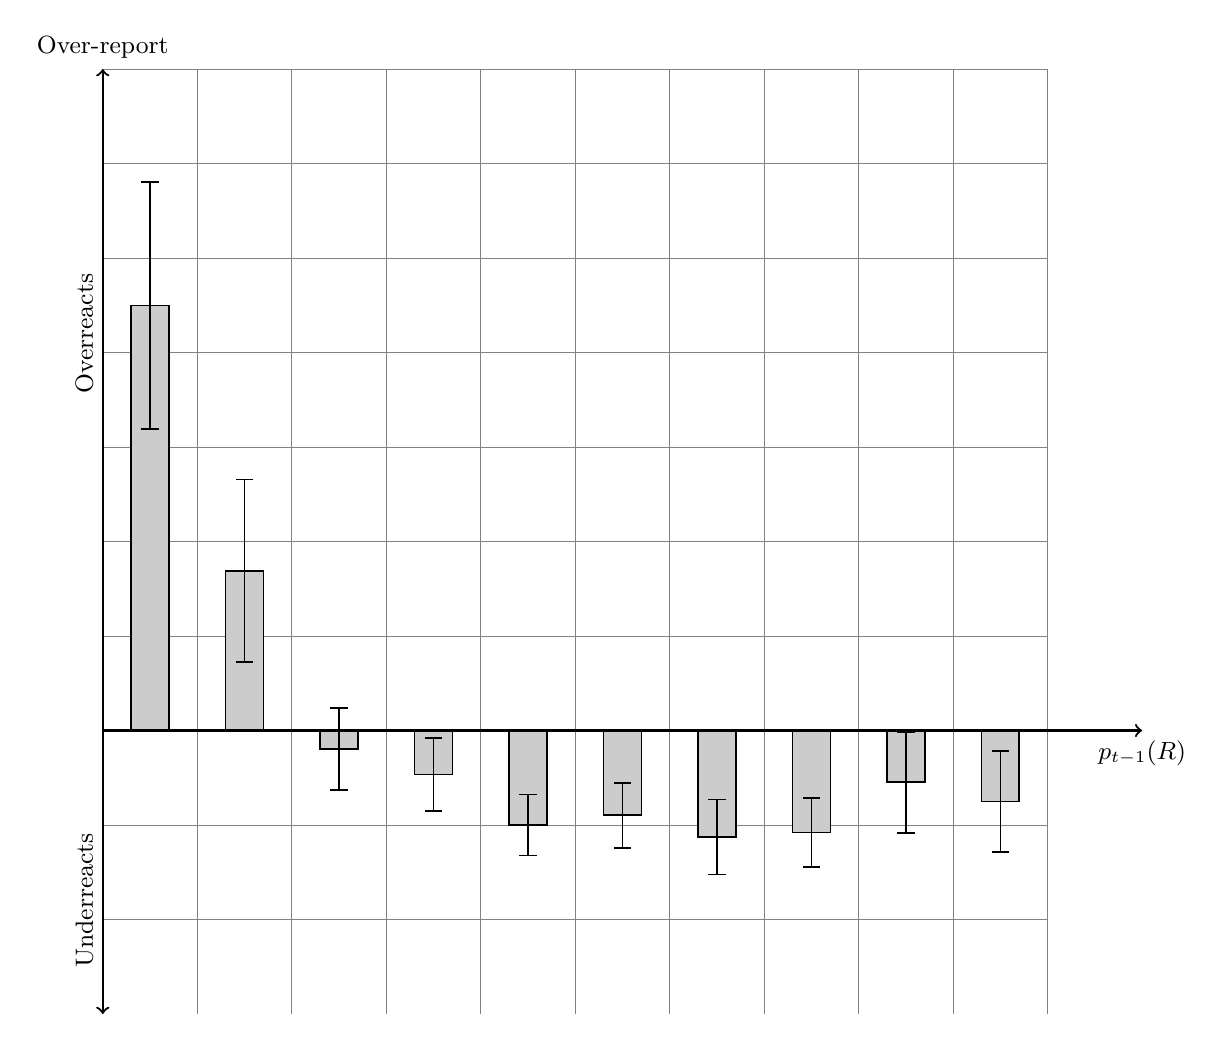
\begin{tikzpicture}[scale=12]
\draw[help lines,step=0.1] (0,-0.3) grid (1,0.7);
\filldraw[opaque,white!80!black] (0.03,0) rectangle (0.07,0.4497);
\draw[line width=0.6] (0.03,0) rectangle (0.07,0.4497);
\draw[line width=0.6,|-|] (0.05,0.3179) -- (0.05,0.5814);
\filldraw[opaque,white!80!black] (0.13,0) rectangle (0.17,0.1691);
\draw[line width=0.6] (0.13,0) rectangle (0.17,0.1691);
\draw[line width=0.6,|-|] (0.15,0.0716) -- (0.15,0.2666);
\filldraw[opaque,white!80!black] (0.23,0) rectangle (0.27,-0.0195);
\draw[line width=0.6] (0.23,0) rectangle (0.27,-0.0195);
\draw[line width=0.6,|-|] (0.25,-0.0636) -- (0.25,0.0246);
\filldraw[opaque,white!80!black] (0.33,0) rectangle (0.37,-0.0466);
\draw[line width=0.6] (0.33,0) rectangle (0.37,-0.0466);
\draw[line width=0.6,|-|] (0.35,-0.0863) -- (0.35,-0.0068);
\filldraw[opaque,white!80!black] (0.43,0) rectangle (0.47,-0.1000);
\draw[line width=0.6] (0.43,0) rectangle (0.47,-0.1000);
\draw[line width=0.6,|-|] (0.45,-0.1333) -- (0.45,-0.0667);
\filldraw[opaque,white!80!black] (0.53,0) rectangle (0.57,-0.0897);
\draw[line width=0.6] (0.53,0) rectangle (0.57,-0.0897);
\draw[line width=0.6,|-|] (0.55,-0.1250) -- (0.55,-0.0544);
\filldraw[opaque,white!80!black] (0.63,0) rectangle (0.67,-0.1127);
\draw[line width=0.6] (0.63,0) rectangle (0.67,-0.1127);
\draw[line width=0.6,|-|] (0.65,-0.1531) -- (0.65,-0.0723);
\filldraw[opaque,white!80!black] (0.73,0) rectangle (0.77,-0.1079);
\draw[line width=0.6] (0.73,0) rectangle (0.77,-0.1079);
\draw[line width=0.6,|-|] (0.75,-0.1455) -- (0.75,-0.0703);
\filldraw[opaque,white!80!black] (0.83,0) rectangle (0.87,-0.0548);
\draw[line width=0.6] (0.83,0) rectangle (0.87,-0.0548);
\draw[line width=0.6,|-|] (0.85,-0.1092) -- (0.85,-0.0004);
\filldraw[opaque,white!80!black] (0.93,0) rectangle (0.97,-0.0751);
\draw[line width=0.6] (0.93,0) rectangle (0.97,-0.0751);
\draw[line width=0.6,|-|] (0.95,-0.1296) -- (0.95,-0.0206);
\draw[line width=0.8,->]  (0,0) -- (1.1,0) node[below] {\small{$p_{t-1}(R)$}};
\draw[line width=0.8,<->] (0,-0.3) -- (0,0.7) node[above] {\small{Over-report}};
\draw (0,0.42) node[above,rotate=90] {\small{Overreacts}};
\draw (0,-0.18) node[above,rotate=90] {\small{Underreacts}};
% ADD THEORY CURVE BELOW
\end{tikzpicture}
